% ASE anonymous review submission layout.
\documentclass[sigconf,screen]{acmart}

\settopmatter{
  printacmref=true,
  printccs=true,
  printfolios=false
}

\copyrightyear{2026}
\acmYear{2026}
\setcopyright{cc}
\setcctype{by}
\acmConference[AgenticDev '26]{The International Workshop on Agentic AI for Next-Generation Software Development }{October 12--16, 2026}{Munich, Germany}
\acmBooktitle{The International Workshop on Agentic AI for Next-Generation Software Development (AgenticDev '26), October 12--16, 2026, Munich, Germany}
\acmDOI{10.1145/3843282.3843716}
\acmISBN{979-8-4007-2985-0/2026/10}
% \setcopyright{none}
% \acmConference[AgenticDev 2026]{International Workshop on Agentic AI for Next-Generation Software Development}{October 12, 2026}{Munich, Germany}
% \acmYear{2026}
% \copyrightyear{2026}
% \acmISBN{}
% \acmDOI{}

\usepackage{booktabs}
\usepackage{graphicx}
\usepackage{microtype}
\microtypesetup{expansion=false}
\usepackage{url}
\usepackage{xspace}
\usepackage{amsmath}
\usepackage{tikz}
\usetikzlibrary{arrows.meta,positioning,calc}

\usepackage{listings}
\definecolor{diffadd}{RGB}{0,110,0}
\definecolor{diffdel}{RGB}{170,0,0}
\lstdefinestyle{trace}{
  basicstyle=\ttfamily\footnotesize,
  columns=fullflexible,
  keepspaces=true,
  breaklines=true,
  breakindent=1.5em,
  frame=single,
  framerule=0.3pt,
  escapechar=|,
  morecomment=[f][\color{diffadd}]{+},
  morecomment=[f][\color{diffdel}]{-},
}

\graphicspath{{figures/}}
\newcommand{\tool}{\textsc{Extender}\xspace}
\newcommand{\etal}{{\em et al.}\xspace}
\newcommand{\ie}{{\em i.e.},\xspace}
\newcommand{\eg}{{\em e.g.},\xspace}
\newcommand{\etc}{{\em etc.}}

\begin{CCSXML}
<ccs2012>
 <concept>
  <concept_id>10011007.10011074.10011075.10011080</concept_id>
  <concept_desc>Software and its engineering~Software maintenance tools</concept_desc>
  <concept_significance>500</concept_significance>
 </concept>
 <concept>
  <concept_id>10010147.10010178.10010199.10010202</concept_id>
  <concept_desc>Computing methodologies~Multi-agent planning</concept_desc>
  <concept_significance>500</concept_significance>
 </concept>
</ccs2012>
\end{CCSXML}
\ccsdesc[500]{Software and its engineering~Software maintenance tools}
\ccsdesc[500]{Computing methodologies~Multi-agent planning}

\begin{document}

\title{\tool: A Multi-Agent System for Code Extensibility Review}
\author{Jiahe Chen}
\affiliation{%
  \institution{Duke Kunshan University}
  \city{Kunshan}
  \state{Jiangsu}
  \country{China}
}

\author{Jiacheng Shen}
\affiliation{%
  \institution{Duke Kunshan University}
  \city{Kunshan}
  \state{Jiangsu}
  \country{China}
}

\begin{abstract}
Software systems must evolve as requirements and environments change, which makes extensibility a central quality goal.
The SOLID principles, \ie five object-oriented design principles, are widely endorsed in software engineering practice to evaluate software quality.
However, automatically detecting violations of SOLID principles remains difficult since many violations are latent design flaws that only surface when the code must be extended.
In this paper, we propose to check the violations of SOLID principles by explicitly extending and checking the extensibility of existing code.
Based on this idea, we design \tool, a multi-agent system that detects SOLID violations by generating principle-specific extension requirements, asking AI agents to implement them, and checking whether the resulting diffs expose design defects.
Experimental results show that \tool achieves \textbf{87.9\%} detection accuracy with a Qwen3.5 9B model, which is 32.1 points higher than the state-of-the-art LLM-based approaches.
\end{abstract}

\keywords{Multi-Agent Systems, SOLID Principles, Software Extensibility}

\maketitle

\section{Introduction}\label{sec:intro}

Software extensibility is a central quality attribute since software usually evolves with requirements, users, and development environments.
The SOLID principles give developers widely used guidance for preserving extensibility.  
They constrain coupling, responsibility boundaries, interfaces, and dependencies~\cite{Martin2000,Martin2017,Ampatzoglou2019,Yanakiev2025}.

Automatically detecting SOLID violations is thus an important research topic that has gained wide attention~\cite{Sharma2018,Palomba2015,
Oktafiani2018,Chebanyuk2016,Martins2024,Pehlivan2025}.
Specifically, existing approaches fall into two categories, \ie code-analysis-based approaches and LLM-based approaches.
The former apply static analysis to extract structural information and code metrics, and detect violations with predefined rules or thresholds over these syntactic proxies~\cite{Sharma2018,Palomba2015,Oktafiani2018, Chebanyuk2016,Roy2024}.
The latter instead rely on the semantic code understanding and reasoning capability of large language models (LLMs) to judge whether the code conforms to each principle~\cite{Martins2024, Pehlivan2025}.

However, existing approaches suffer from poor accuracy in detecting SOLID violations~\cite{Martins2024,Pehlivan2025}.
The root cause lies in the fact that they detect SOLID principle violations purely based on the current state of the code.
In contrast, violations of SOLID principles depend on the cost of a future change.
A design can look acceptable before it is challenged, and its defect becomes visible only when a new variant or dependency is introduced.
Since existing approaches reason only over the current version of the code, they cannot measure the cost to be is paid when the code is extended.


In this paper, we propose \tool, a multi-agent system that detects SOLID violations by explicitly extending the code under review.
Our key idea is to organize SOLID violation detection as a multi-agent extension experiment.
Specifically, \tool consists of four types of agents.
A \textit{manager} first creates five constrained code extension requests, one for each SOLID principle.
Five parallel \textit{engineers} then implement the requests on isolated copies of the input code.
For each extended code, an \textit{analyst} checks whether the difference between each extended version and the original code matches a principle-specific violation pattern.
Finally, a \textit{ranker} aggregates the analysis results and returns the most likely violations together with all supporting artifacts.

We evaluate \tool with Qwen3.5 9B on a SOLID violation detection dataset~\cite{Pehlivan2025} and compare it with two LLM-based baselines~\cite{Pehlivan2025,Melo2025}, \ie a single-agent baseline and a two-agent baseline under a detector-evaluator paradigm~\cite{Melo2025}. 
\tool reaches 87.9\% top-2 accuracy, which is 17.9 and 32.1 points higher than the single-agent and two-agent baselines.
These results validate that explicitly extending the code exposes latent design flaws that facilitate SOLID violation detection.

This paper makes three contributions:
\begin{itemize}
  \item We are the first to propose adopting agent-based code extension to expose latent design flaws in code for detecting SOLID principle violations. 
  \item We implement and open-source \tool, a multi-agent system for code extensibility review\footnote{https://github.com/jiahe-chen/extender}. 
  \item We evaluate \tool on real-world SOLID violation detection datasets and show that \tool can effectively improve detection accuracy by up to 32.1\% compared with the state-of-the-art one-agent and two-agent baselines.
\end{itemize}

\section{Background \& Related Work}\label{sec:related}

This section defines the design principles studied in this work and distinguishes traditional, LLM-based, and agentic approaches to code quality evaluation.

\begin{figure*}[!t]
  \vspace*{-6pt}
  \centering
  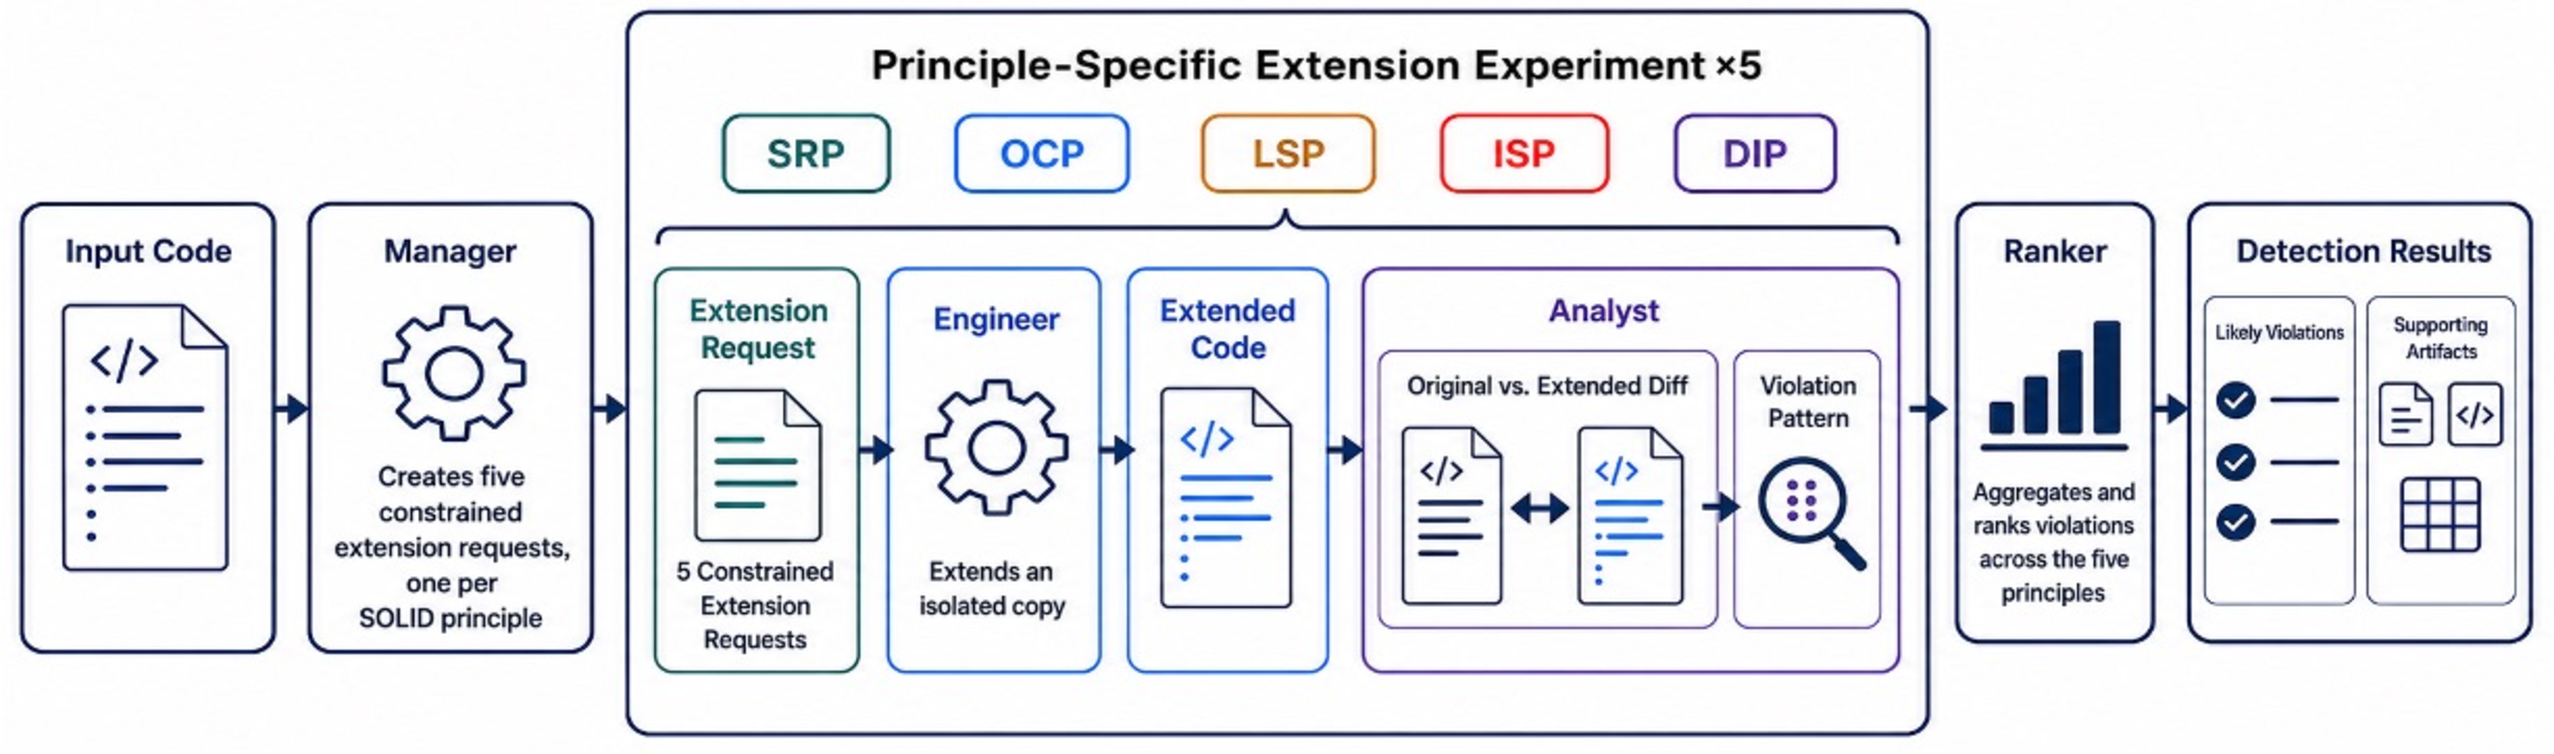
\includegraphics[width=\textwidth]{figures/extender_workflow.pdf}
  \vspace{-0.2in}
  \caption{The \tool multi-agent workflow.}\label{fig:architecture}
  \vspace{-0.1in}
\end{figure*}

\subsection{SOLID Principles}
SOLID principles are widely adopted in industry to improve code modularity and maintainability~\cite{Ampatzoglou2019,Turan2018,Yanakiev2025}.
They comprise five object-oriented design principles~\cite{Martin2000,Martin2017}.
Specifically, the \textbf{Single Responsibility Principle (SRP)} limits a module to implement only one responsibility.
The \textbf{Open/Closed Principle (OCP)} favors adding new behavior through extension instead of modifying existing stable code that is extensively tested.
The \textbf{Liskov Substitution Principle (LSP)} requires subtypes to preserve the behavior of their base types, which ensures that the newly implemented subtypes can correctly replace any parent references in existing systems.
The \textbf{Interface Segregation Principle (ISP)} prevents clients from depending on operations they do not use, which reduces the overhead of implementing dumb interfaces when extending the code.
Finally, the \textbf{Dependency Inversion Principle (DIP)} makes high-level policy depend on abstractions rather than concrete implementations to simplify code extension.

These principles protect extensibility by reducing the impact of potential bugs induced by code changes.  
A violation is therefore not only a property of the current source structure.  
It often becomes observable when a new variant, subtype, client, or dependency forces unexpected edits.



\subsection{Traditional Code Quality Evaluation}
Traditional code-quality tools use static rules, source metrics, and structural proxies to identify code smells and design problems~\cite{Sharma2018,Palomba2015}.
For SOLID, existing techniques check class diagrams, coupling relationships, interface structure, and explicit dispatch logic~\cite{Oktafiani2018,Chebanyuk2016,Roy2024}.
These analyses are deterministic, repeatable, and inexpensive enough for continuous integration.  
Refactoring studies also assess SOLID indirectly by measuring a system before and after manual design improvements~\cite{Ampatzoglou2019,Yanakiev2025}.

However, existing static indicators only work when a violation has a clear structural signature.
They cannot reliably recover architectural intent or the cost of a change that has not yet been attempted.  
Traditional evaluation thus describes the current program well, but it does not directly test how the program responds to a targeted extension.



\subsection{LLM-Based SOLID Violation Detection}
LLMs extend code analysis beyond fixed syntactic rules by using learned representations of programs and natural-language design knowledge~\cite{Chen2021,Roziere2024,Guo2024,Fan2023}.
Recent work applies this capability to design-pattern recognition and software-quality assessment~\cite{AzimHassan2024,Martins2024}.  
For SOLID specifically, Martins et al. use an LLM to enforce principles during code review~\cite{Martins2024}.
Pehlivan et al. systematically evaluate prompts and code models on a multilingual benchmark covering all five principles~\cite{Pehlivan2025}.

While existing LLM-based approaches improve semantic coverage, they still ask a model to infer a future design problem from the current code snapshot.
Their accuracy consequently varies across principles, especially when a violation becomes visible only after the code is extended.  
Compared with existing LLM-based approaches, \tool changes the evidence available to the model by first generating a targeted extension and then analyzing the resulting difference in code.

\subsection{Agentic Approaches to Code Quality}

Agentic systems divide a complex task among roles for planning, acting, reflection, and coordination~\cite{Wang2024,Yao2023}.  
In code-quality evaluation, prior tools combine static rules, machine learning, IDE assistance, or LLM feedback to detect and sometimes refactor test smells~\cite{Aljedaani2021,Pontillo2024,Wang2021,Lambiase2020,Lucas2024}.
Melo et al. show that a detector-evaluator workflow can identify and refactor test smells with small language models~\cite{Melo2025}.

\tool also assigns specialized agent roles, but organizes them for a different purpose.
Existing agentic tools divide the detection task itself among roles, \eg a detector and an evaluator that reason over the program as given~\cite{Melo2025}.
The agents in \tool instead cooperate to conduct a controlled extension experiment that produces the diff evidence discussed above, and each finding remains traceable to the extension request and the modified lines that produced it.

\begin{table*}[t]
  \centering
  \caption{Code extension requirements and violation patterns for each SOLID principle.}\label{tab:patterns}
  \vspace{-0.1in}
  \small
  \begin{tabular}{p{0.08\textwidth}p{0.39\textwidth}p{0.43\textwidth}}
    \toprule
    \textbf{Principles} & \textbf{High-Level Requirement Generation Instructions} & \textbf{Principle Violation Patterns} \\
    \midrule
    SRP & Change one architectural layer. & The diff crosses independent layers,
    such as controller or view. \\
    OCP & Add a type, variant, or case. & The extension edits an existing
    \texttt{if-else} or \texttt{switch} branch. \\
    LSP & Exercise parent and subtype behavior polymorphically. & A subtype throws
    or breaks the contract expected from the parent. \\
    ISP & Implement only a needed subset of an interface. & The implementation is
    forced to add unused methods. \\
    DIP & Replace one concrete dependency. & The high-level module must edit several concrete references. \\
    \bottomrule
  \end{tabular}
  \vspace{-0.1in}
\end{table*}

\section{The \tool Multi-Agent System}\label{sec:method}

\subsection{System Overview}
In this paper, we propose \tool, a multi-agent system that detects violations in SOLID principles by explicitly extending the code under review.
As shown in Figure~\ref{fig:architecture}, \tool has four agents in a workflow.
On receiving input code, it invokes a \textit{manager} to create five constrained code extension requirements, one for each SOLID principle.
Five parallel \textit{engineers} then extend isolated code copies for each requirement.
Given the extended code by each engineer, an \textit{analyst} compares the extension with the original code and checks whether the code difference matches a principle-specific violation pattern.
Finally, a \textit{ranker} aggregates the analysis results and returns the most likely violations together with all supporting artifacts.
Such a design enables us to adopt the difference between the original code and extended code to detect code extensibility issues, \ie violations of SOLID principles, which can expose more latent design errors in the current code base.

In the rest of this section, we first introduce the detailed design of each agent.
We then demonstrate a working example of SOLID violation detection with our system.
Finally, we will briefly discuss our implementation. 


\subsection{Agent Design}
In this subsection, we introduce the detailed design of the four agents of \tool respectively.

\subsubsection{Manager}
The \textit{manager} is responsible for creating a concrete extension requirement for each SOLID principle.
Since the input code varies from case to case, we design a high-level requirement generation instruction for each principle to expose the specific code design flaws.
The second column of Table~\ref{tab:patterns} shows our high-level instructions. 
The \textit{manager} then instantiates them into a code-specific requirement.

Specifically, for \textbf{SRP}, we instruct the \textit{manager} to design an extension requirement that modifies only one architectural layer.
Code with potential \textbf{SRP} violations can then involve changes in other layers.
For \textbf{OCP}, the high-level instruction is to add a new type, variant, or case to the current implementation.
Code with \textbf{OCP} violations may potentially modify existing code rather than adding new code.
For \textbf{LSP}, the instruction is to exercise the parent type and its subtypes polymorphically.
Code with \textbf{LSP} violations can expose bugs when using subtypes in applications designed for parent types.
For \textbf{ISP}, the instruction is to implement only a needed subset of an existing interface.
Code that violates \textbf{ISP} may then be forced to carry methods it does not need.
Finally, for \textbf{DIP}, the instruction is to replace one concrete dependency with an alternative.
A violation can be detected by checking whether the high-level module is edited due to missing abstractions.

\subsubsection{Engineer}
Given the requirement generated by the \textit{manager}, a dedicated \textit{engineer} implements it and produces a revised program. 
We isolate \textit{engineers} for each SOLID principle to reduce the context length of each agent since agents with long contexts usually result in suboptimal results~\cite{Levy2024SameTask}.

\subsubsection{Analyst}
The \textit{analyst} is responsible for detecting SOLID violations for each principle based on the code extension requirement, the original code, and the revised code.
For each principle, a verdict that indicates whether the principle is violated and a reason are generated.
Specifically, the \textit{analyst} first computes a unified $\operatorname{diff}$ between the extended program and the original code with a deterministic textual diff tool.
It then checks whether the $\operatorname{diff}$ matches the violation pattern configured for the target principle.

The violation patterns are summarized in the third column of Table~\ref{tab:patterns}.
For \textbf{SRP}, the \textit{analyst} checks whether the change requested within a single architectural layer spreads into other layers.
For \textbf{OCP}, the \textit{analyst} reports a violation when the new variant edits an existing \texttt{if-else} or \texttt{switch} branch, instead of adding new code along an extension point.
For \textbf{LSP}, the \textit{analyst} flags a violation whenever a subtype throws an exception or otherwise breaks the contract expected from its parent under polymorphic calls.
For \textbf{ISP}, the \textit{analyst} confirms a violation whenever the new implementation is forced to carry unused methods or \texttt{NotImplementedError} stubs.
Finally, for \textbf{DIP}, the \textit{analyst} reports a violation whenever replacing one concrete dependency forces edits in the high-level module because no useful abstraction is present.

\subsubsection{Ranker}
Finally, the \textit{ranker} aggregates the five verdicts into the detection result in a single call.
Given the original program and the verdicts from all principles, the \textit{ranker} first discards the principles with negative decisions or unsatisfied structural prerequisites.
It then ranks the remaining candidate violations by how evident they are, considering two criteria: (1)~the clarity of the evidence, and (2)~the strength of the explanation.
The \textit{ranker} reports the top-$k$ candidates ($k{=}2$ by default) as the most likely violations.
Each candidate is accompanied by its supporting artifacts, including the extension requirement, the $\operatorname{diff}$, and the \textit{analyst}'s explanation.
Developers can trace every reported violation back to the request and the modified lines that produced it.

\subsection{A Working Example}

Listing~\ref{lst:ocp25} shows an example from an actual run of \tool on the benchmark code \texttt{OCP\_25}.
The original code calculates the area of various shapes, \ie the \texttt{AreaCalculator} class dispatches on concrete shape types with a \texttt{when} expression.
\begin{lstlisting}[
  style=trace,
  float=t,
  captionpos=b,
  belowskip=-5pt,
  caption={\tool on benchmark sample \texttt{OCP\_25}.},
  label={lst:ocp25}
]
|\textbf{Manager}| -> requirement |$r_{\mathrm{OCP}}$|:
  "Add support for a Triangle shape to the area calculation system."
   
|\textbf{Engineer}| -> diff |$d_{\mathrm{OCP}}$| (abridged):
+ class Triangle(private val base: Double,
+   private val height: Double) : Shape("Triangle") {...}
  class AreaCalculator {
    fun calculateArea(shape: Shape): Double {
      return when (shape) {
        is Rectangle -> shape.getWidth() * shape.getHeight()
        is Circle -> Math.PI * shape.getRadius() * ...
+       is Triangle -> 0.5 * shape.getBase() * ...
        else -> 0.0}}}
        
|\textbf{Analyst}| -> verdict |$v_{\mathrm{OCP}}$|: violation detected
  "The AreaCalculator class violates the Open/Closed Principle because its calculateArea() method contains a conditional block (when expression) that directly handles specific shape types. ... This structure requires modifying the existing decision logic ... rather than extending the system through new polymorphic types or dedicated handlers."
   
|\textbf{Ranker}| -> top-2: [OCP, DIP]
  "OCP: adding a new shape requires modifying this existing method ... DIP: depending on concrete implementations ... rather than an abstraction." (ground truth: OCP, reported at rank 1)

\end{lstlisting}

The trace shows how the four agents cooperate on a concrete input. 
Given the high-level OCP instruction, the \textit{manager} instantiates it into a code-specific requirement, \ie adding support for a \texttt{Triangle} shape to the area calculation system.
The \textit{engineer} adds a \texttt{Triangle} class and edits the existing \texttt{when} branch inside \texttt{AreaCalculator.calculateArea}, which violates OCP.
The \textit{analyst} accordingly returns a positive verdict and explains that accommodating new shapes requires modifying the existing decision logic instead of extending the system through new polymorphic types.
The \textit{ranker} finally arbitrates among the channels.
In this example, the SRP, ISP, and DIP channels also return positive verdicts, and the \textit{ranker} places OCP first and DIP second because their explanations identify the most clearly located evidence.

% This example illustrates what the extension experiment adds beyond directly pointing at a visible conditional: the generated diff demonstrates the exact edit required by a realistic new variant, and the reported violation remains traceable to the requirement, the modified lines, and the \textit{analyst} explanation that produced it.
\subsection{Implementation}
\tool is implemented as a LangGraph state machine~\cite{LangGraph2024}.
The backbone LLM can be integrated either through a local Ollama server~\cite{Ollama2024} or any cloud provider.
The evaluated configuration runs Qwen3.5 9B locally~\cite{Qwen2025}, and unified diffs are computed deterministically with Python's \texttt{difflib}.

In our implementation, we use five channels, each responsible for one SOLID principle.
For each channel, we record the output for each agent in the entire workflow.
Because the channels are mutually independent, \textit{engineer} execution can be parallelized in deployment, and a failed or malformed extension is retained as an inconclusive artifact without blocking the remaining channels.
The full system and analysis scripts are packaged for release.

\section{Evaluation}\label{sec:evaluation}
\subsection{Experimental Setup}
We evaluate \tool on the SOLID benchmark of Pehlivan et al.~\cite{Pehlivan2025}.
It contains 240 labeled examples, 48 for each principle. 
The 240 examples span four programming languages, \ie Java, Kotlin, Python, and C\#, and three difficulty levels, \ie easy, moderate, and hard.
There are 60 examples for each programming language and 80 examples for each difficulty.
Each example has one ground-truth violation label.

We compare \tool with two baseline workflows.
A one-agent baseline directly prompts an LLM to identify a violation, which is proposed by Pehlivan \etal~\cite{Pehlivan2025}.  
A two-agent baseline uses a detector agent and an evaluator agent for up to three feedback iterations.  
The two-agent baseline is originally proposed by Melo \etal~\cite{Melo2025} for code smell detection. 
We revise their prompt to make it work for SOLID violation detection.
All three workflows use the same Qwen3.5 9B model deployed on a desktop with an NVIDIA GeForce RTX 4060 GPU.  

For each example, all workflows receive the same source code and return a ranked list of SOLID labels.  
We configure the systems to return two labels because code can exhibit related design symptoms, while the benchmark supplies one primary label.  
We preserve the original runs and use fixed configurations for the reported comparison.  
The one-agent and two-agent baselines have access to the same principle definitions as \tool.
The difference is that they reason directly over the source and their conversational context rather than a set of generated extension diffs.

\subsection{Metrics}
Throughout this paper, accuracy refers to top-2 accuracy, \ie a prediction is correct when the ground-truth violation appears in the first two ranked results.
We therefore define accuracy as:

\begin{equation}
  \text{Accuracy} = \frac{1}{N}\sum_{i=1}^{N}
  \mathbf{1}[y_i \in \{\hat{y}^{(1)}_i,\hat{y}^{(2)}_i\}].
\end{equation}

We also report Mean Reciprocal Rank (MRR@2) and Macro-F1.  
MRR@2 rewards systems that place the correct result first.  
For Macro-F1, we adopt a resolved prediction to comply with the top-2 accuracy.
Specifically, when the ground-truth label appears in the returned pair, that hit is resolved to the ground-truth class.
Otherwise, the first valid prediction is used.  

\begin{figure}[t]
  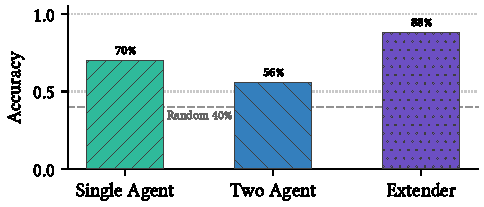
\includegraphics[width=0.9\columnwidth]{paper_fig_overall.pdf}
  \vspace{-0.1in}
  \caption{Overall accuracy on 240 examples.}\label{fig:overall}
  \vspace{-0.1in}
\end{figure}


% \begin{table}[t]
%   \centering\small
%   \caption{Performance of different workflows.}\label{tab:overall}
%   \vspace{-0.05in}
%   \begin{tabular}{lccc}
%     \toprule
%     \textbf{System} & \textbf{Accuracy} & \textbf{MRR@2} & \textbf{Macro-F1} \\
%     \midrule
%     One Agent  & 70.00\% & 0.638 & 0.699 \\
%     Two Agent  & 55.83\% & 0.490 & 0.576 \\
%     \textbf{\tool } & \textbf{87.92\%} & \textbf{0.792} & \textbf{0.888} \\
%     \bottomrule
%   \end{tabular}
% \end{table}

\subsection{Main Results}


Figure~\ref{fig:overall} shows that \tool improves accuracy by 17.9 points over the one-agent baseline and by 32.1 points over the two-agent baseline.  
The gain in MRR@2 (Table~\ref{tab:overall}) shows that the multi-agent system also ranks correct results higher.  
The Macro-F1 score confirms that its improvement is not limited to one principle.


\begin{table}[t]
  \centering\small
  \caption{Performance of different workflows.}\label{tab:overall}
  \vspace{-0.05in}
  \begin{tabular}{lccc}
    \toprule
    \textbf{System} & \textbf{Accuracy} & \textbf{MRR@2} & \textbf{Macro-F1} \\
    \midrule
    One Agent  & 70.00\% & 0.638 & 0.699 \\
    Two Agent  & 55.83\% & 0.490 & 0.576 \\
    \textbf{\tool } & \textbf{87.92\%} & \textbf{0.792} & \textbf{0.888} \\
    \bottomrule
  \end{tabular}
  \vspace{-0.1in}
\end{table}

\begin{figure}[t]
  \centering
  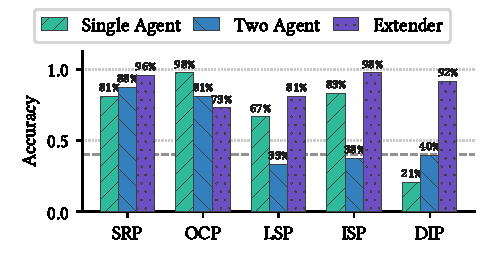
\includegraphics[width=0.97\columnwidth]{paper_fig_violation.pdf}
  \vspace{-0.1in}
  \caption{Accuracy by different principles.}\label{fig:principles}
  \vspace{-0.1in}
\end{figure}

\noindent
\textbf{\textit{Analysis on each principle.}}
\tool leads on SRP, LSP, ISP, and DIP~\cite{Martin2000,Martin2017} (Figure~\ref{fig:principles}).
Compared with the two baselines, \tool improves most on DIP.  
This is because tight coupling becomes clear when an \textit{engineer} attempts to replace a concrete dependency.  
However, \tool has suboptimal accuracy on OCP.  
This is because a direct prompt can often recognize a visible dispatch branch without an extension experiment.

\noindent
\textbf{\textit{Analysis on different difficulty levels.}}
\tool remains at 80\% on Hard examples (Figure~\ref{fig:difficulty}).
This is because the \textit{analyst} receives a focused $\operatorname{diff}$ rather than all generated context.
This helps the multi-agent system concentrate on modifications that carry review evidence.
It also reduces the impact of long source inputs.

\noindent
\textbf{\textit{Analysis on more powerful LLMs.}}
We also compare \tool with the single-agent baseline on more powerful LLMs on the cloud.
Specifically, we use Qwen3.5 Plus with 397 billion parameters, which is over $44\times$ larger than the Qwen3.5 9B model used by \tool.
As shown in Table~\ref{tab:cloud}, \tool can achieve over 92\% of the performance compared with on-cloud LLMs, despite the huge gap in model capabilities.
This result shows that \tool is a strong lever for independent developers to deploy a smaller model on their own devices to conduct high-accuracy code review, significantly reducing API cost for development and code review.
% The development cost can be thus significantly reduced.

% \begin{table}[t]
%   \centering\small
%   \caption{\tool (Local) against a cloud baseline.}\label{tab:cloud}
%   \vspace{-0.05in}
%   \begin{tabular}{lccc}
%     \toprule
%     \textbf{System} & \textbf{Accuracy} & \textbf{MRR@2} & \textbf{Macro-F1} \\
%     \midrule
%     One Agent (Qwen3.5 9B) & 70.00\% & 0.638 & 0.699 \\
%     \textbf{\tool (Qwen3.5 9B)} & \textbf{87.92\%} & \textbf{0.792} & \textbf{0.888} \\
%     One Agent (Qwen3.5 Plus) & 95.83\% & 0.858 & 0.960 \\
%     \bottomrule
%   \end{tabular}
% \end{table}



\section{Discussion and Future Work}\label{sec:discussion}

\textbf{\textit{Generality.}}
We argue that \tool is a general paradigm for code extensibility review rather than a tool for detecting SOLID principle violations.
The key idea is to adopt the extend-then-detect paradigm to detect code extensibility issues.
Since individual principles in SOLID enter the workflow only as a pair of natural-language artifacts, any design rule whose defect manifests as resistance to change can be plugged in by defining a new pair. However, one limitation is that the paradigm is best suited to scenarios where an extension is genuinely needed to expose a latent design flaw.
This is confirmed by the fact that \tool underperforms the direct prompt on OCP, whose violations often carry a visible syntactic symptom.
In the future, we plan to add a lightweight \textit{router} in front of the workflow that predicts whether a violation is already detectable from the current state of the code.

\begin{table}[t]
  \centering\small
  \caption{\tool (Local) against a cloud baseline.}\label{tab:cloud}
  % \vspace{-0.05in}
  \begin{tabular}{lccc}
    \toprule
    \textbf{System} & \textbf{Accuracy} & \textbf{MRR@2} & \textbf{Macro-F1} \\
    \midrule
    One Agent (Local 9B) & 70.00\% & 0.638 & 0.699 \\
    One Agent (Cloud 397B) & 95.83\% & 0.858 & 0.960 \\
    \tool (Local 9B) & 87.92\% & 0.792 & 0.888 \\
    \bottomrule
  \end{tabular}
\end{table}


\begin{figure}[t]
  \centering
  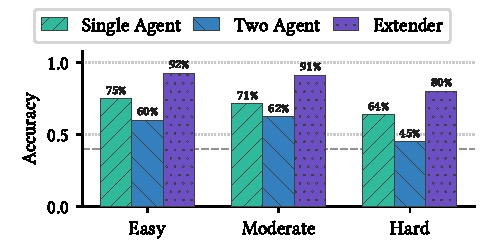
\includegraphics[width=0.97\columnwidth]{paper_fig_difficulty.pdf}
  \vspace{-0.1in}
  \caption{Accuracy by difficulty.}\label{fig:difficulty}
  \vspace{-0.1in}

\end{figure}

\noindent
\textbf{\textit{Explainability.}}
\tool is designed for strong explainability.
The \textit{manager} request, the \textit{engineer} extension, the executed $\operatorname{diff}$, the \textit{analyst} verdict, and the final rationale from the \textit{ranker} are all recorded.
Developers can trace a finding to the exact changed lines and accept or reject it on evidence.
The same trace also separates planning, generation, and analysis errors, which turns a wrong finding into a diagnosable event instead of an opaque failure. In the future, we plan to close the loop with reviewer feedback to evolve the performance of \tool.
Specifically, when a developer rejects a finding, the recorded trace identifies the responsible stage, so the corresponding instruction or violation pattern can be refined automatically rather than by global prompt tuning.

\noindent
\textbf{\textit{Repository-scale evaluation.}}
Our evaluation follows the curated benchmark of Pehlivan \etal~\cite{Pehlivan2025}, in which each example is a self-contained snippet with a single ground-truth label.
This small-scale setting is what enables a controlled comparison across workflows.
However, we are aware that the small-scale benchmark bounds the conclusions we can draw since real-world violations often span multiple files and entangle several principles at once.
In the future, we plan to extend \tool to repository-level datasets to evaluate our extend-then-detect paradigm in a more realistic setting.


\noindent
\textbf{\textit{Computational cost and request realism.}}
All experiments were conducted locally on a desktop equipped with a consumer-grade GPU. 
Our implementation executes the five principle-specific channels sequentially and is therefore intended for asynchronous code review rather than real-time editor feedback. 
In the future, we will extend our code to support parallel code extension to improve computational efficiency.
% The generated requests are intended as controlled extensibility probes rather than predictions of actual future requirements. 
% They are tailored to the input code and represent common maintenance operations, while their similarity to requests from real projects remains to be evaluated.

\section{Conclusion}
In this paper, we identify that the key limitation of existing SOLID violation detection approaches lies in that they reason only over the current state of the code, while many violations are latent design flaws that surface only when the code must be extended.
We propose an extend-then-detect paradigm, which leverages the code understanding and software development capabilities of LLMs to actually extend the code under review before judging it.
Based on this idea, we design \tool, a multi-agent system for code extensibility review, in which four agents cooperate to turn each SOLID principle into a concrete extension experiment and detect violations via differences in code.
Experimental results show that \tool can effectively outperform the one-agent and two-agent baselines by 17.9 and 32.1 points, respectively.

\clearpage
\bibliographystyle{ACM-Reference-Format}
\bibliography{main}

\end{document}